\documentclass[12pt]{article}

\usepackage{sbc-template}
\usepackage{graphicx,url}
\usepackage{amsmath}
\usepackage{amssymb}

\usepackage{indentfirst}
\usepackage{listings}
\usepackage{algorithm}
\floatname{algorithm}{Algoritmo}
\usepackage{algorithmicx}
\usepackage{algpseudocode}
% \usepackage[portuguese]{algorithm2e}
\usepackage[T1]{fontenc}
\usepackage[utf8]{inputenc}  
\usepackage[brazil]{babel}

\usepackage{tikz}
\usetikzlibrary{shapes.multipart,positioning,arrows,calc}
\tikzset{
  listnode/.style={
    rectangle split,rectangle split parts=2,draw,rectangle split horizontal,fill=blue!20
  },
  startnode/.style={
    draw,minimum width=1.5cm,minimum height=.75cm
  }
}

\usepackage[edges]{forest} % draw trees

\sloppy

\title{Estruturas de Dados e Projetos de Algoritmos\\Tutores (URI 2120)}
\author{Fabrício S. Paranhos\inst{1} e Leandro A. Vianna\inst{1}}
\address{Instituto de Informática -- Universidade Federal de Goiás (UFG)}

\begin{document} 

\maketitle

% \begin{abstract}
%   This meta-paper describes the style to be used in articles and short papers
%   for SBC conferences. For papers in English, you should add just an abstract
%   while for the papers in Portuguese, we also ask for an abstract in
%   Portuguese (``resumo''). In both cases, abstracts should not have more than
%   10 lines and must be in the first page of the paper.
% \end{abstract}
     
\begin{resumo} 
  No desenvolvimento de uma solução para associar tutores a alunos Lucca
  Siaudzionis fornece uma solução elegante: utilizar uma árvore binária de busca
  aonde os alunos são representado por nós e seus tutores são seus respectivos
  pais na árvore. Entretanto, devido a problemas técnicos, reconstruir a mesma
  torna-se impraticável, com complexidade de inserção na ordem O($n$).
  Desenvolvemos um novo algoritmo, capaz de lidar com as demandas e limitações
  temporais do problema, com o auxílio de uma árvore binária balançeada
  auxiliar, com inserção de complexidade O($\lg n$). Permitindo a consulta aos
  tutores sem a necessidade de armazenamento da árvore binária de busca. 
\end{resumo}

\section{Descrição do Problema (Tutores - URI 2120)} \label{sec:tutores}

O problema Tutores\footnote{\url{https://www.urionlinejudge.com.br/judge/en/problems/view/2120}}
consiste em dado uma ordem de inserções de chaves em uma Árvore
Binária de Busca (ABB), deve ser respondido para várias chaves qual a chave do nó
pai do nó em que essa chave está.

Formalmente, dado uma ordem de inserção de chaves $O = \{X_1, X_2, \cdots, X_n\}$ e
uma ABB $T$ em que foram inseridas as chaves $O$. Considere $p(X)$ como a chave
do nó pai do nó em que a chave $X$ está em $T$. Para uma sequência $I = \{i_1, i_2, \cdots, i_m\}$,
a solução deve apresentar uma sequência de resposta $Y = \{p(X_{i_1}), p(X_{i_2}), \cdots, p(X_{i_m})\}$.

Por exemplo, suponhamos a ordem $\hat{O} = \{2, 4, 5, 6, 1\}$ e a sequência $\hat{I} = \{2, 3, 4\}$.
A sequência de resposta é $Y = \{p(X_2 = 4) = 2, p(X_3 = 5) = 4, p(X_4 = 6) = 5\}$. Os valores
de $p$ podem ser visualizados na árvore binária de busca $T$ desse exemplo que 
está na figura \ref{fig:abb_exemplo}.

\begin{figure}[!htb]
\centering
\begin{forest}
for tree={
    grow=south,
    circle, draw, minimum size=3ex, inner sep=1pt,
    s sep=7mm
        }
[2
	[1]
	[4
		[5
			[6]
		]
	]
]
\end{forest}
\caption{Árvore Binária de Busca $T$ gerada a partir da ordem de inserção de chaves $\hat{O}$}
\label{fig:abb_exemplo}
\end{figure}
\section{Resultados} \label{sec:res}
% 
\subsection{Estruturas de Dados}
\label{sec:estruturas}

\subsubsection{Splay Tree}
\label{sec:splay}


% \subsubsection{Hash table}
% \label{sec:hash}

% Tabela \textit{hash}, ou embaralhamento, é uma estrutura de dado que permite
% associar uma \textit{key} (chave) a um valor. As principais características
% dessa estrutura de dados são: inserção e busca com complexidade O(1). Sua
% implementação utiliza uma matriz unidimensional de tamanho fixo.
% Para determinar a posição de inserção de uma chave $k$ na matriz utiliza-se
% uma função de embaralhamento (\textit{hash}).

% A função \textit{hash} ($h: A \rightarrow \text{\texttt{int}}$) deve ser
% uniforme, ou seja, distribuir uniformemente as chaves do tipo $A$ entre os
% índices da matriz unidimensional, e possuir complexidade O(1).
% Não existe função de embaralhamento universalmente ideal, por isso cada tipo de
% dado ($A$) possui uma específica.

% Inevitavelmente, conflitos irão surgir ($\exists a~b: A,~ h(a) = h(b)~\text{com}
% ~a \neq b$), por
% dois motivos: como comentado anteriormente a função de embaralhamento
% não é perfeita e a quantidade de dados inseridos é maior que a tabela. Uma forma
% de resolver conflitos é utilizar baldes (\textit{buckets}) para armazenar chaves
% com conflitos, através da uma lista ligada com inserção na cabeça da lista,
% como representado na figura~\ref{fig:hash}, dessa forma obtendo inserção O(1).
% Para garantirmos a segunda condição da tabela de embaralhamento (busca em O(1))
% dependemos da uniformidade da função \textit{hash} e do tamanho inicial da
% tabela, ou quantidade de baldes.

% Neste trabalho, os elementos da tabela são pares de números inteiros (\textit{key}:
% \texttt{int}, \textit{val}: \texttt{int}), portanto utilizamos a função módulo
% tamanho da tabela ($N$) como função de embaralhamento ($h(key) = key \text{\texttt{\%}} N$),
% o que garante uma distribuição relativamente uniforme das matrículas com complexidade O(1).

% \begin{figure}[!htb]
%   \centering
%   \begin{tikzpicture}[scale=.2, >=stealth]
%     \node[startnode] (t0) {T[0]};
%     \node[startnode,below=0pt of t0] (t1) {T[1]};
%     \node[startnode,below=0pt of t1] (t2) {T[2]};
%     \node[listnode,right=of t0] (3) {3};
%     \node[listnode,right=of t1] (1) {1};
%     \node[listnode,right=.5cm of 1] (7) {7};
%     \node[listnode,right=of t2] (2) {2};
%     \node[listnode,right=.5cm of 2] (5) {5};
%     \node[listnode,right=.5cm of 5] (8) {8};
%     \node[right=.5cm of 3] (3x) {$\varnothing$};
%     \node[right=.5cm of 7] (7x) {$\varnothing$};
%     \node[right=.5cm of 8] (8x) {$\varnothing$};
%     \draw[*->] let \p1 = (3.two), \p2 = (3.center) in (\x1,\y2) -- (3x);
%     \draw[*->] let \p1 = (1.two), \p2 = (1.center) in (\x1,\y2) -- (7);
%     \draw[*->] let \p1 = (7.two), \p2 = (7.center) in (\x1,\y2) -- (7x);
%     \draw[*->] let \p1 = (2.two), \p2 = (2.center) in (\x1,\y2) -- (5);
%     \draw[*->] let \p1 = (5.two), \p2 = (5.center) in (\x1,\y2) -- (8);
%     \draw[*->] let \p1 = (8.two), \p2 = (8.center) in (\x1,\y2) -- (8x);
%     \draw[->] (t0) edge (3) (t1) edge (1) (t2) edge (2);
%   \end{tikzpicture}

%   \caption{Representação da tabela \textit{hash} com três \textit{buckets}
%     implementados utilizando listas ligadas.}
%   \label{fig:hash}
% \end{figure}
\subsection{Algoritmo} \label{sec:algo}
Pela descrição do problema, para definir os tutores de cada aluno o sistema
utiliza uma Árvore Binária de Busca (ABB), em que o pai do aluno na árvore é seu
tutor. Entretanto, o custo da inserção seria proibitivo se utilizássemos a mesma
estrutura para encontrar os tutores, que no pior caso, seria uma árvore
binária degenerada com complexidade de inserção e busca $O(n)$.

Observa-se que a ABB define uma sequência de matrículas
relacionada a um determinado percurso e a estrutura da árvore. Nossa solução (algoritmo~\ref{alg:parent}) propõe 
modelar a mesma sequência, entretanto utilizando uma árvore binária balanceada auxiliar
para calcular os pais e altura dos alunos em relação a ABB original.

Como a árvore binária balanceada auxiliar foi escolhido utilizar a \textit{Splay Tree}, que não tem garantia de uma árvore com altura $O(\lg n)$, mas a complexidade amortizada de $O(m \lg n)$ para uma sequência de $m$ operações. Para guardar os pais e alturas dos alunos na ABB foi escolhido a \textit{Hash Table} com tratamento de colisão por encadeamento.

\begin{algorithm}[ht]
  \small
  \caption{Calcula o pai (tutor) de cada matrícula, modelando a sequência \textit{inorder} de uma Árvore Binária de Busca (ABB) utilizando uma árvore binária balanceada.}
  \label{alg:parent}
  \begin{algorithmic}[1]
    \Require $mat[N]$ vetor de matrículas de tamanho $N$; $parent$ tabela \textit{hash}.
    \Procedure{Parents}{$mat[N], parent$}% \Comment{Vetor de matrículas de tamanho $N$.}
    % \State $keys[N] \gets 0$\Comment{Vetor de chaves com tamanho $N$.}
    \State $order \gets$ \Call{SplayTree}{ }
    % \State $parent \gets$ \Call{HashTable}{N}
    \State $level \gets$ \Call{HashTable}{N}

    \Statex
    \For{$i \gets 0, N-1$}
    % \State $keys[i] \gets mat[i]$

    \If{$order \neq \emptyset$}
    \State \Call{ParentsInner}{$mat$, $parent$, $order$, $level$}
    \EndIf \Comment{$order \neq \emptyset$}
    \Statex
    
    \State \Call{Insert}{$order, mat[i]$}
    % \State $i \gets i + 1$
    
    \EndFor
    \EndProcedure
  \end{algorithmic}
\end{algorithm}

\begin{algorithm}[ht]
  \small
  \caption{Procedimento interno de \textsc{Parents}.}
  \label{alg:parent_inner}
  \begin{algorithmic}[1]
    \Require $mat[N]$ vetor de matrículas de tamanho $N$; $parent$ tabela \textit{hash}.
    \Procedure{ParentsInner}{$mat$, $parent$, $order$, $level$}
    \State $upper \gets$ \Call{LowerBound}{$order, mat[i]$}
    \Statex
    \If{$upper$ not found}
    % \State // Matrículas são menores que $mat[i]$. Sequência ord.: $\ldots
    % W X$
    % \Statex
    \State $w \gets$ \Call{Max}{$order$} \Comment{Maior elemento de $order$.}
    \State $l \gets$ \Call{LookUp}{$level, w+1$} \Comment{$l = level[w+1]$}
    \State \Call{Insert}{$parent, mat[i], w$} \Comment{$parent[mat[i]] = w$}
    \State \Call{Insert}{$level, mat[i], l$}
    \Statex
    \ElsIf{$upper = $ \Call{Min}{$order$}} \Comment{Menor elemento de $order$}
    % \State // Matrículas são maiores que $x$. Sequência ord.: $X W
    % \ldots$
    % \State $w \gets$ \Call{Min}{$order$}
    \State $l \gets$ \Call{LookUp}{$level, upper+1$}
    \State \Call{Insert}{$parent, mat[i],upper$}
    \State \Call{Insert}{$level, mat[i],l$}
    \Statex
    \Else
    \State $lower \gets$ \Call{Previous}{$order, upper$} \Comment{Elemento anterior em $order$}
    \Statex
    % \State // $lower$ e $upper$ estão no meio. Sequência ord.: $\ldots~ L ~
    % X ~ U ~\ldots$
    % \Statex
    % \State // $upper$ é o pai? $upper$ está na subárvore de $lower$?
    \If{\Call{LookUp}{$level, upper$} $>$ \Call{LookUp}{$level, lower$}}
    \State $l \gets$ \Call{LookUp}{$level, upper$}
    \State \Call{Insert}{$parent, mat[i], upper$}
    \State \Call{Insert}{$level, mat[i], l+1$}
    \Statex
    \Else
    % \State // $lower$ é o pai? $lower$ está na subárvore de $upper$?
    \State $l \gets$ \Call{LookUp}{$level, lower$}
    \State \Call{Insert}{$parent, mat[i], lower$}
    \State \Call{Insert}{$level, mat[i], l+1$}
    \EndIf
    \EndIf \Comment{$upper$ not found}
    
    \EndProcedure
  \end{algorithmic}
\end{algorithm}

O algoritmo recebe uma lista de matrículas ($mat$) e uma tabela ($parent$) associando alunos e
tutores vazia. Inicialmente definimos uma \textit{Splay Tree} ($order$), aonde
serão feitas as inserções das matrículas, e outra tabela ($level$) associando a matrícula à
altura na árvore original, linhas 2 e 3. Após a inicialização, percorremos todos
os alunos (linha 4), simulando o percurso original (procedimento \textsc{ParentsInner}) e finalmente
inserimos na árvore balanceada (linha 29).

Dentro do procedimento \textsc{ParentsInner} queremos
encontrar qual posição da sequência a matrícula $i$ ($mat[i]$) encaixará,
para isso procuramos (linha 2) pela menor matrícula ($upper$) tal que seja maior
ou igual à matrícula $i$ ($mat[i]$) na árvore $order$. Caso a matrícula ($upper$) não
exista, podemos concluir que nossa sequência terá o seguinte formato após inserção: $(\ldots,
w,mat[i])$, ou seja $mat[i]$ é maior que todas as matrículas na ABB e filho de $w$. Assim obtemos o maior elemento da sequência ($w$ linha
4) e a altura ($l$) na qual $mat[i]$ seria inserido na árvore (linha 5),
finalmente atualizamos as tabelas de pais e alturas com os novos dados de $mat[i]$
(linhas 6--7). Caso a matrícula exista ($upper$) ela pode ser o primeiro
elemento da sequência (linhas 8--11), isto é a menor matrícula, ou estar em qualquer posição no
meio da sequência (linhas 12--23). Se $upper$ for o menor elemento da árvore
$order$, a sequência terá formato: $(mat[i], w, \ldots)$, ou seja, $mat[i]$ é a
menor matrícula na árvore original com pai $upper$. Analogamente, obtemos a altura ($l$) na qual
$mat[i]$ seria inserido e atualizamos a tabela de pais e alturas (linhas 10--11).
Para o último caso teríamos sequência de formato: $(\ldots, lower, mat[i],
upper, \ldots)$, em que $lower$ é a matrícula anterior a $upper$ em $order$
(linha 13).
\begin{figure}[!htb]
\centering
% dot -Gdpi=300 -Tpng test1.dot > test1.png
%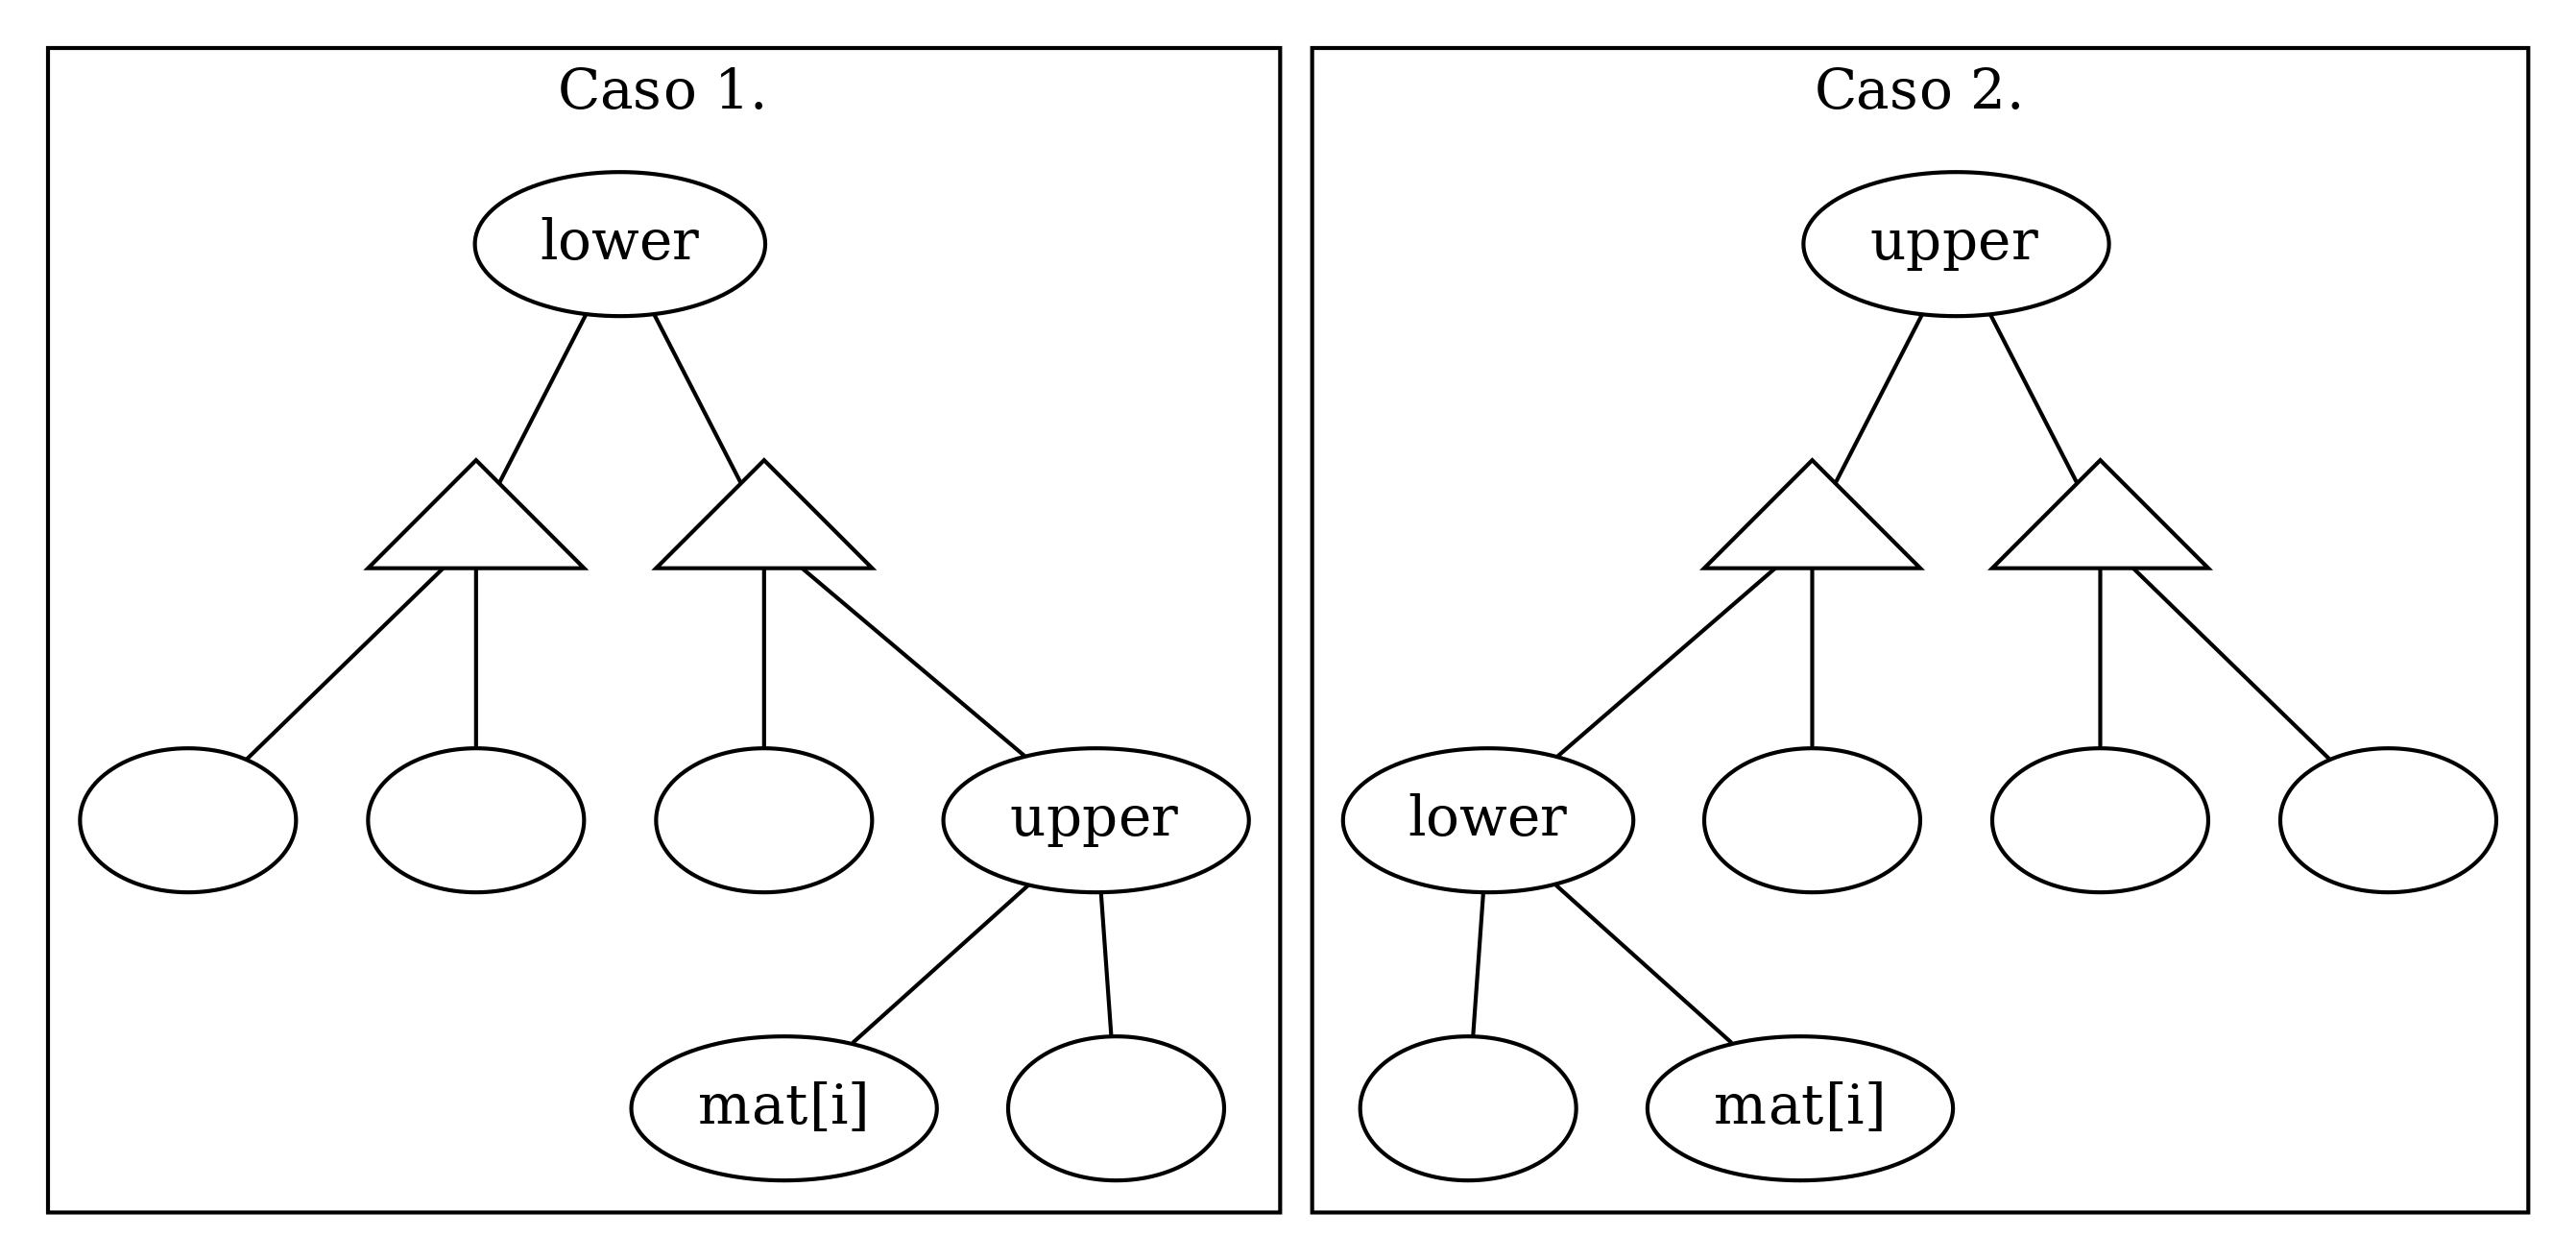
\includegraphics[width=0.7\linewidth]{lxu.png}

\begin{forest}
[$lower$, ellipse
	[$\cdots$, fit=band]
	[$\cdots$, edge=dashed
		[, phantom]
		[$upper$, ellipse, edge=dashed
			[{$mat[i]$}]
			[$\cdots$, edge=dashed]
		]
	]
]
\node at (current bounding box.south)    [below=1ex,draw,rectangle]{Caso 1};
\end{forest}
\hspace{1em}
\begin{forest}
[$upper$, ellipse
	[$\cdots$, edge=dashed
		[$lower$, ellipse, edge=dashed
			[$\cdots$, edge=dashed]
			[{$mat[i]$}]
		]
		[, phantom]
	]
	[$\cdots$, fit=band]
]
\node at (current bounding box.south)    [below=1ex,draw,rectangle]{Caso 2};
\end{forest}

\caption{Se $mat[i]$ será inserido entre duas matrículas na sequência, existem dois casos para a estrutura da ABB.}
\label{fig:lxu}
\end{figure}

Nesse passo temos duas configurações possíveis, como pode ser visto
na figura~\ref{fig:lxu}, portanto precisamos determinar quem está na subárvore
de quem (linha 14) para escolher a configuração correta: se $upper$ está na subárvore de $lower$ (caso 1) então $upper$ é pai de $mat[i]$ (linhas 15--17), caso contrário (caso 2) $lower$ é pai de $mat[i]$ (linhas 19--21). Ao final do algoritmo a
tabela $parent$ possui os tutores de cada aluno.

\subsubsection{Análise da complexidade}
As operações \textsc{Max}, \textsc{Min}, \textsc{Previous},
\textsc{Insert}($parent$) e \textsc{Insert}($level$), inserção em tabela
\textit{hash}, possuem complexidade O(1), enquanto a operação
\textsc{LowerBound} é O($\lg n$), em que $n$ é a quantidade de elementos na árvore. Como discutido na seção~\ref{sec:algo}
a operação \textsc{Insert}($order$), utilizando análise amortizada, possui
complexidade O($m \lg n$), para $m$ operações. Analogamente, por análise amortizada, a operação
\textsc{LookUp}, de uma tabela \textit{hash} com tratamento de colisão por
encademaneto, possui complexidade O(1). Com isso, os trechos 3--7, 8--11 e
12--21 possuem complexidade O(1), então o bloco entre 3--24 tem complexidade O(1). Concluímos,
portanto que a complexidade do algoritmo \textsc{Parents} é, pela aproximação de
Stirling:
\begin{align*}
  \sum_{i = 1}^{N}(\text{O}(\lg i) + \text{O}(1) + \text{O}(\lg i)) = \sum_{i = 1}^{N}(\text{O}(\lg i)) = \text{O}(\lg \prod_{i = 1}^{N} i) = \text{O}(\lg N!) \sim N \lg N
      % ~\text{O}(n \lg n)
\end{align*}
\subsection{Casos de Teste}\label{sec:testes}
Nessa seção demostraremos alguns exemplos de casos de teste do problema Tutores e qual o comportamento da \textit{Splay Tree} ao realizar a inserção das matrículas.

\subsubsection{Exemplo de Caso de Teste 1}
\begin{lstlisting}[frame=single,caption=Instância de teste 1,label=test1,escapeinside={\%*}{*)},inputencoding=utf8]
  3     // %*Número de estudantes*)
  5 1 2 // %*Ordem de inserção dos estudantes*)
  1     // %*Quantas consultas serão realizadas*)
  2     // %*Tutor do estudante 2*)
\end{lstlisting}

\begin{figure}[htb]
\centering
% dot -Gdpi=300 -Tpng test1.dot > test1.png
%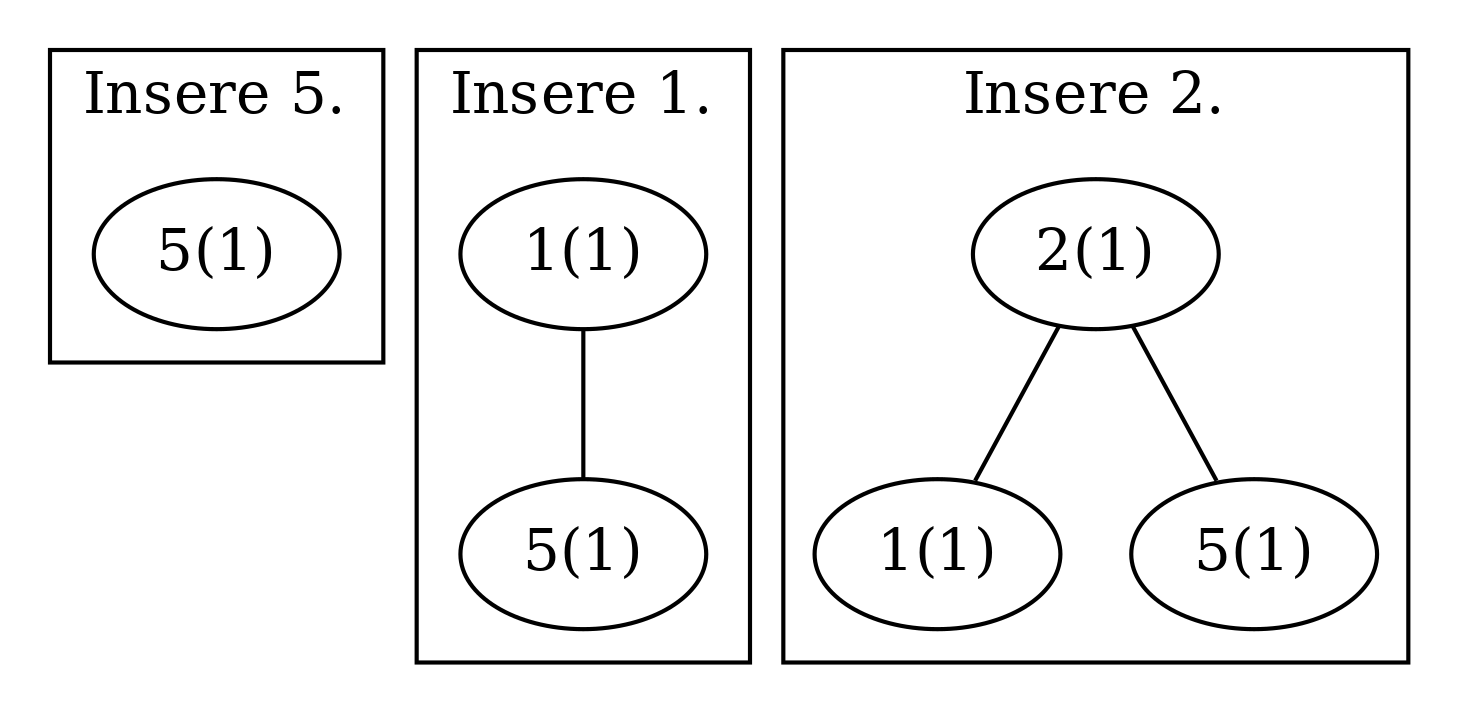
\includegraphics[width=0.5\linewidth]{test1.png}
\begin{forest}
[5
	[$\emptyset$]
	[$\emptyset$]
]
\end{forest}
\hspace{1em}
\begin{forest}
[1
	[$\emptyset$]
	[5
		[$\emptyset$]
		[$\emptyset$]
	]
]
\end{forest}
\hspace{1em}
\begin{forest}
[2
	[1
		[$\emptyset$]
		[$\emptyset$]
	]
	[5
		[$\emptyset$]
		[$\emptyset$]
	]
]
\end{forest}
\caption{\textit{Splay Tree} após cada inserção de chave do Caso de Teste 1}
\label{fig:test1}
\end{figure}

\subsubsection{Exemplo de Caso de Teste 2}
\begin{lstlisting}[frame=single,caption=Instância de teste 1,label=test2,escapeinside={\%*}{*)},inputencoding=utf8]
  5         // %*Número de estudantes*)
  3 1 4 2 5 // %*Ordem de inserção dos estudantes*)
  2         // %*Quantas consultas serão realizadas*)
  2 5       // %*Tutores dos estudantes 2 e 5*)
\end{lstlisting}

\begin{figure}[htb]
\centering
% dot -Gdpi=300 -Tpng test2.dot > test2.png
%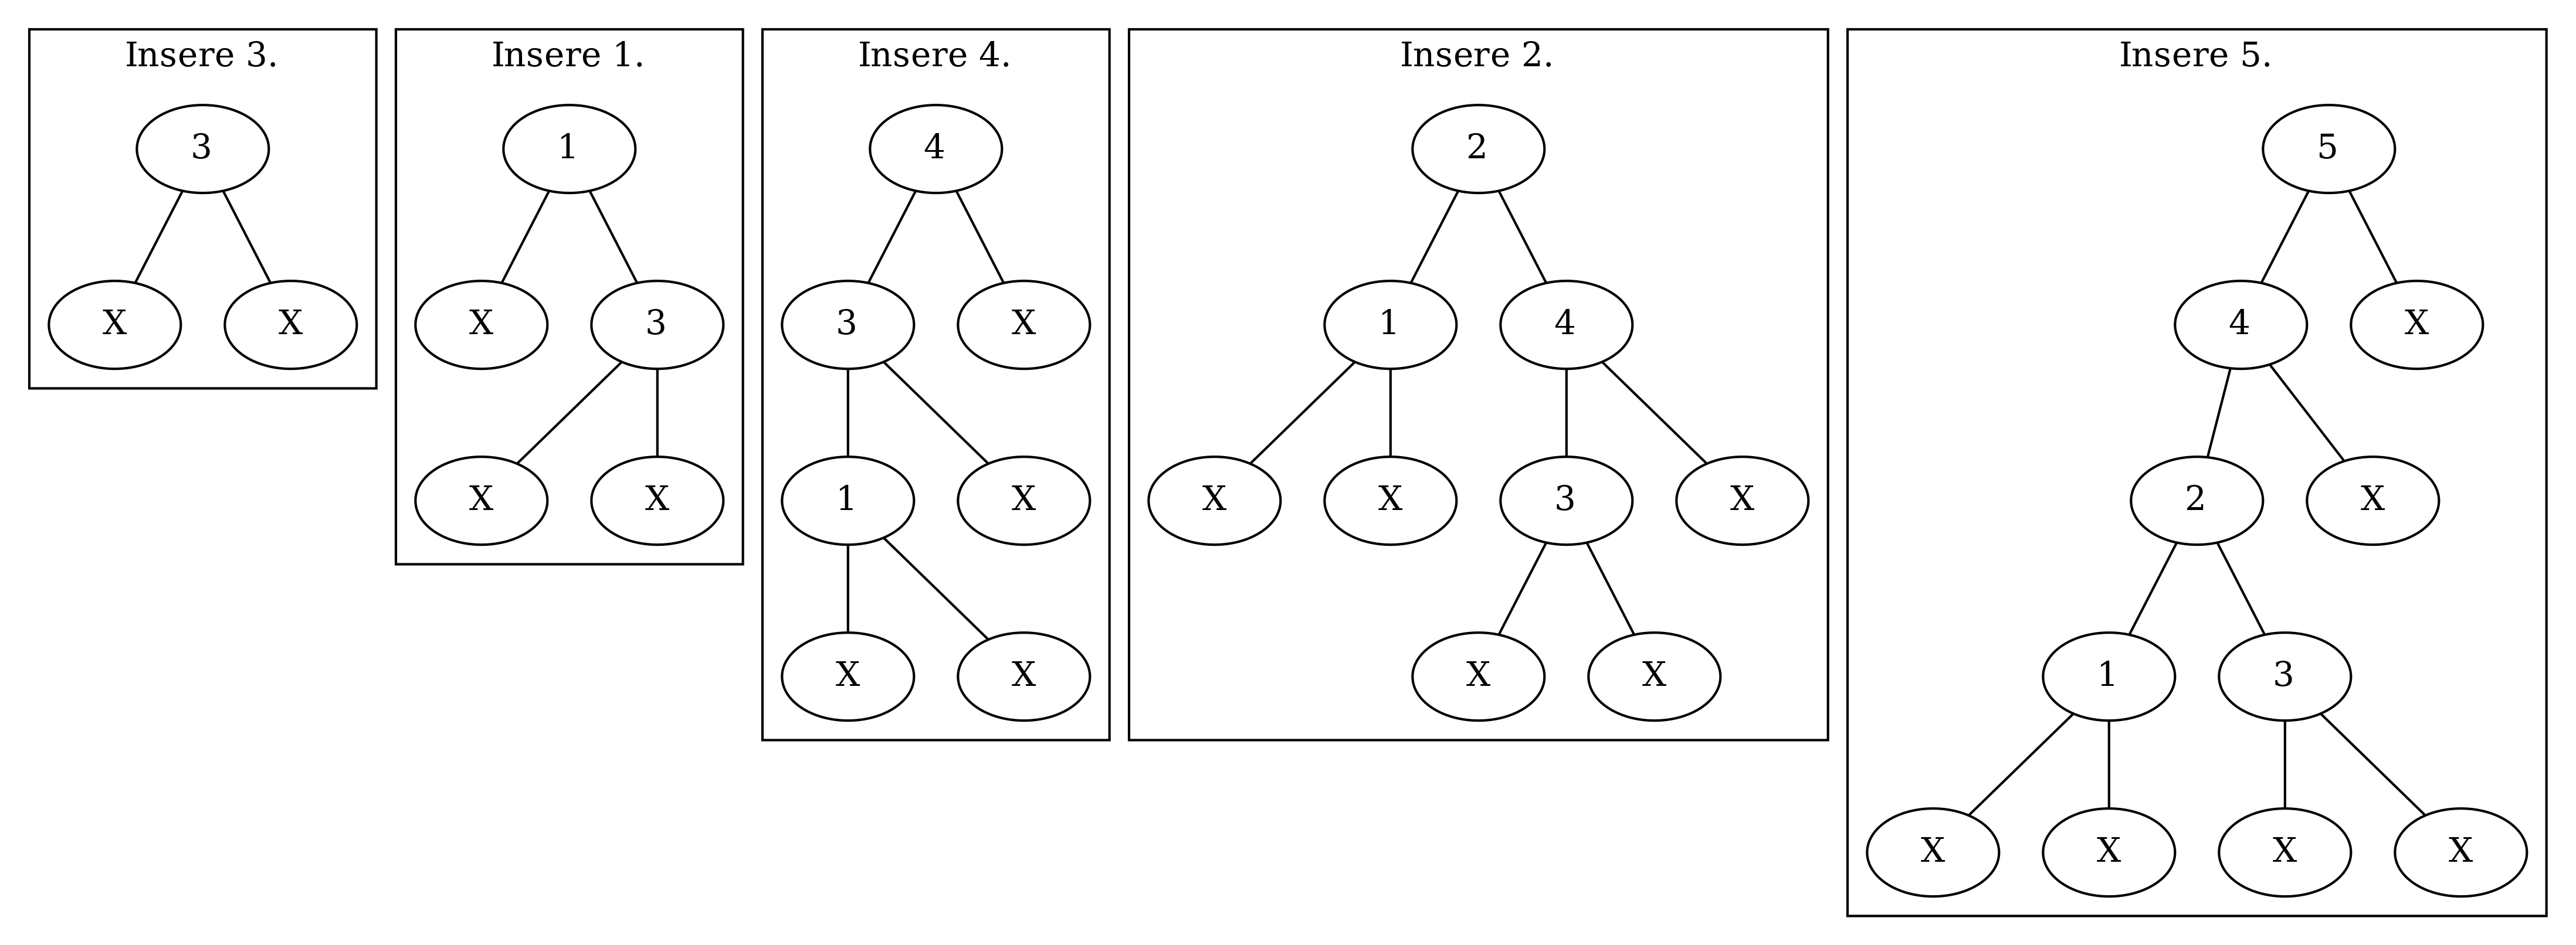
\includegraphics[width=\linewidth]{test2.png}
\begin{forest}
[3
	[$\emptyset$]
	[$\emptyset$]
]
\end{forest}
\hspace{1em}
\begin{forest}
[1
	[$\emptyset$]
	[3
		[$\emptyset$]
		[$\emptyset$]
	]
]
\end{forest}
\hspace{1em}
\begin{forest}
[4
	[3
		[1
			[$\emptyset$]
			[$\emptyset$]
		]
		[$\emptyset$]
	]
	[$\emptyset$]
]
\end{forest}
\hspace{1em}
\begin{forest}
[2
	[1
		[$\emptyset$]
		[$\emptyset$]
	]
	[4
		[3
			[$\emptyset$]
			[$\emptyset$]
		]
		[$\emptyset$]
	]
]
\end{forest}
\hspace{1em}
\begin{forest}
[5
	[4
		[2
			[1
				[$\emptyset$]
				[$\emptyset$]
			]
			[3
				[$\emptyset$]
				[$\emptyset$]
			]
		]
		[$\emptyset$]
	]
	[$\emptyset$]
]
\end{forest}
\caption{\textit{Splay Tree} após cada inserção de chave do Caso de Teste 2}
\label{fig:test2}
\end{figure}

\subsubsection{\textit{Benchmarks}}
Com o objetivo de verificar o tempo de execução, testamos nossa solução com casos de diferentes de tamanhos. São dois tipos de casos em tamanhos de $10$ à $10^5$ com as chaves gerados uniformemente aleatórias:
\begin{itemize}
\item Matrículas em qualquer ordem (não ordenadas).
\item Matrículas \textbf{ordenadas}.
\end{itemize}

Os tempos de execução estão descrito no gráfico da figura \ref{fig:benchmark}.

\begin{figure}[!ht]
\centering
\begin{tikzpicture}[]
\begin{axis}[
	xlabel=Tamanho do Problema,
	ylabel=Tempo de Execução (ms),
	width=11cm,height=7cm,
    legend style={at={(0.0,.91)},anchor=west}
    ]

\addplot[color=red,mark=x] coordinates {
(10, 1)
(100, 1)
(1000, 3)
(10000, 26)
(100000, 322.5)
};

\addplot[color=blue,mark=*] coordinates {
(10, 1)
(100, 1)
(1000, 1)
(10000, 11)
(100000, 104.5)
};

\legend{Não ordenado, Ordenado}
\end{axis}
\end{tikzpicture}
\caption{Tempo de execução em milissegundos para os testes gerados.}
\label{fig:benchmark}
\end{figure}

Se observa um tempo melhor para os casos em que as chaves são adicionadas em \textbf{ordem crescente}, o que pode ser explicado pois a cada inserção o último nó inserido vai estar na raiz da \textit{Splay Tree} (por característica da estrutura de dados) e como esse nó vai ser o pai do nó que está sendo inserido nesse momento, isso acelera a busca por ele.


\section{Conclusões}
\label{sec:conc}

% \section{General Information}

% All full papers and posters (short papers) submitted to some SBC conference,
% including any supporting documents, should be written in English or in
% Portuguese. The format paper should be A4 with single column, 3.5 cm for upper
% margin, 2.5 cm for bottom margin and 3.0 cm for lateral margins, without
% headers or footers. The main font must be Times, 12 point nominal size, with 6
% points of space before each paragraph. Page numbers must be suppressed.

% Full papers must respect the page limits defined by the conference.
% Conferences that publish just abstracts ask for \textbf{one}-page texts.

% \section{First Page} \label{sec:firstpage}

% The first page must display the paper title, the name and address of the
% authors, the abstract in English and ``resumo'' in Portuguese (``resumos'' are
% required only for papers written in Portuguese). The title must be centered
% over the whole page, in 16 point boldface font and with 12 points of space
% before itself. Author names must be centered in 12 point font, bold, all of
% them disposed in the same line, separated by commas and with 12 points of
% space after the title. Addresses must be centered in 12 point font, also with
% 12 points of space after the authors' names. E-mail addresses should be
% written using font Courier New, 10 point nominal size, with 6 points of space
% before and 6 points of space after.

% The abstract and ``resumo'' (if is the case) must be in 12 point Times font,
% indented 0.8cm on both sides. The word \textbf{Abstract} and \textbf{Resumo},
% should be written in boldface and must precede the text.

% \section{CD-ROMs and Printed Proceedings}

% In some conferences, the papers are published on CD-ROM while only the
% abstract is published in the printed Proceedings. In this case, authors are
% invited to prepare two final versions of the paper. One, complete, to be
% published on the CD and the other, containing only the first page, with
% abstract and ``resumo'' (for papers in Portuguese).

% \section{Sections and Paragraphs}

% Section titles must be in boldface, 13pt, flush left. There should be an extra
% 12 pt of space before each title. Section numbering is optional. The first
% paragraph of each section should not be indented, while the first lines of
% subsequent paragraphs should be indented by 1.27 cm.

% \subsection{Subsections}

% The subsection titles must be in boldface, 12pt, flush left.

% \section{Figures and Captions}\label{sec:figs}


% Figure and table captions should be centered if less than one line
% (Figure~\ref{fig:exampleFig1}), otherwise justified and indented by 0.8cm on
% both margins, as shown in Figure~\ref{fig:exampleFig2}. The caption font must
% be Helvetica, 10 point, boldface, with 6 points of space before and after each
% caption.

% \begin{figure}[ht]
% \centering
% 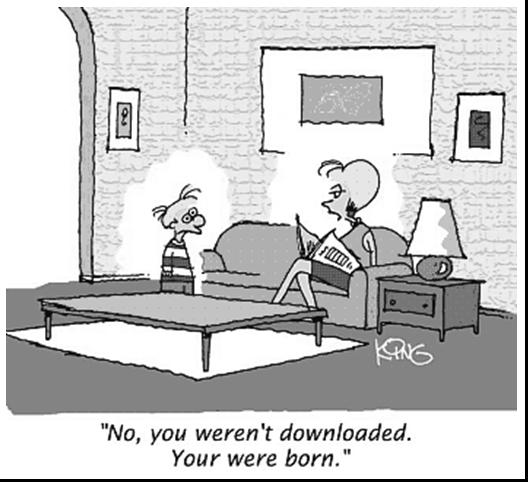
\includegraphics[width=.5\textwidth]{fig1.jpg}
% \caption{A typical figure}
% \label{fig:exampleFig1}
% \end{figure}

% \begin{figure}[ht]
% \centering
% 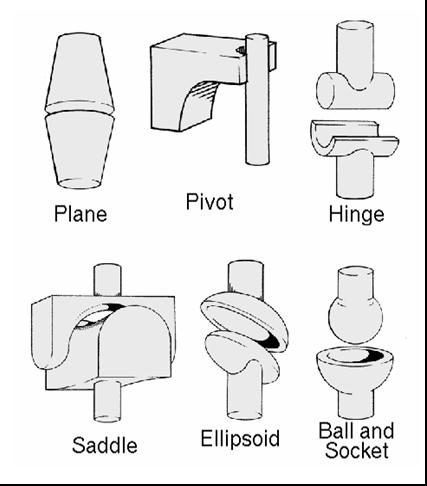
\includegraphics[width=.3\textwidth]{fig2.jpg}
% \caption{This figure is an example of a figure caption taking more than one
%   line and justified considering margins mentioned in Section~\ref{sec:figs}.}
% \label{fig:exampleFig2}
% \end{figure}

% In tables, try to avoid the use of colored or shaded backgrounds, and avoid
% thick, doubled, or unnecessary framing lines. When reporting empirical data,
% do not use more decimal digits than warranted by their precision and
% reproducibility. Table caption must be placed before the table (see Table 1)
% and the font used must also be Helvetica, 10 point, boldface, with 6 points of
% space before and after each caption.

% \begin{table}[ht]
% \centering
% \caption{Variables to be considered on the evaluation of interaction
%   techniques}
% \label{tab:exTable1}
% 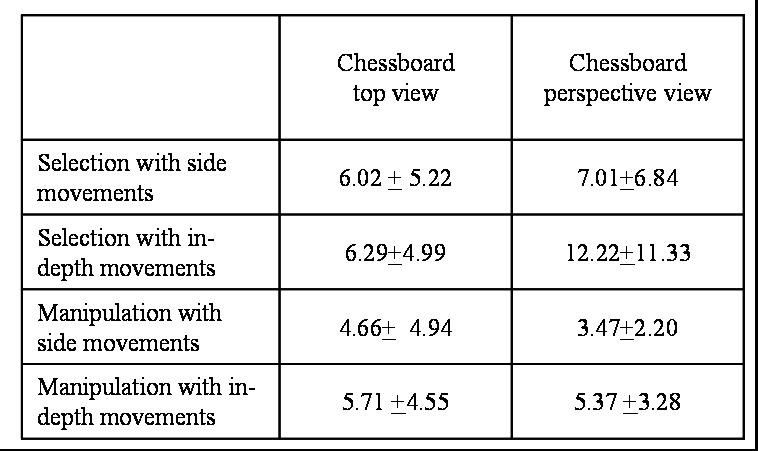
\includegraphics[width=.7\textwidth]{table.jpg}
% \end{table}

% \section{Images}

% All images and illustrations should be in black-and-white, or gray tones,
% excepting for the papers that will be electronically available (on CD-ROMs,
% internet, etc.). The image resolution on paper should be about 600 dpi for
% black-and-white images, and 150-300 dpi for grayscale images.  Do not include
% images with excessive resolution, as they may take hours to print, without any
% visible difference in the result. 

% \section{References}

% Bibliographic references must be unambiguous and uniform.  We recommend giving
% the author names references in brackets, e.g. \cite{knuth:84},
% \cite{boulic:91}, and \cite{smith:99}.

% The references must be listed using 12 point font size, with 6 points of space
% before each reference. The first line of each reference should not be
% indented, while the subsequent should be indented by 0.5 cm.

\bibliographystyle{sbc}
\bibliography{sbc-template}

\end{document}
